\documentclass[openany]{book}

\usepackage{generalsnips}
\usepackage{calculussnips}
\usepackage[margin = 1in]{geometry}
\usepackage{pdfpages}
\usepackage[spanish]{babel}
\usepackage{amsmath}
\usepackage{amsthm}
\usepackage[utf8]{inputenc}
\usepackage{titlesec}
\usepackage{xpatch}
\usepackage{fancyhdr}
\usepackage{tikz}
\usepackage{hyperref}
\title{Pensamiento Político Contemporáneo}
\date{2020 July 30} % , 08:37AM
\author{David Corzo} % Gabriel Mcmath

\begin{document}
\maketitle
%%%%%%%%%%%%%%%%%%%%%%%%%%%%%%%%%%%%%%%%%%%%%%%%%%%%%%%%%%%%%%%%%%%%%%%%%%%%%%%%%%%%%%%%%%%%%%%%%%%%%%%%%%%%%%%%%%%%%%%%%%%%%%%%%%%%%%%%%%%%%%

\chapter{Primera unidad}
\section{Orígenes de six sigma}
\begin{itemize}
    \item Desarrollado después de la segunda guerra mundial. 
        \begin{itemize}
            \item Los alemanes botaban un barco y los aliados tenían 4 barcos más, los aliados botaban un barco de los alemanes el barco era preciado. 
            \item Six Sigma viene de la demanda a producir en masa de la segunda guerra mundial. 
        \end{itemize}

    \item Precursoras directas TQM \& SPC. 
    \item 1987 - Motorola. 
    \item Resultados: incremento en productividad 12.3\% anual. Reducción de costos de no calidad 84\%, eliminación 99.7\% defectos de proceso, ahorros en costo sobre \$10 mio, 17\% crecimiento anual sobre ganancias, ingresos valor de acciones. Motorola asegura haber ahorrado \$1,000 mío desde su implementación.
    \item \pregunta{Cómo desacelero un proceso} 
    \item Kaizen es simple observation.
    \item Six sigma está enfocado en la calidad, es una métrica. 
\end{itemize}

\subsection{Six sigma $6\sigma$}
Metodología de mejora de procesos, centrada en la reducción de la variabilidad de los mismos, consiguiendo reducir o eliminar los defectos o fallas en la entrega de un producto o servicio al cliente. 

\section{Pruebas de hipótesis}
\begin{itemize}
    \item Asumimos que $\mu=\mu_0$ (hipótesis nula).
        \begin{itemize}
            \item Esto significa que estoy asumiendo que existe una campana de Gauss.
        \end{itemize}
        \begin{figure}[H]
            \centering
            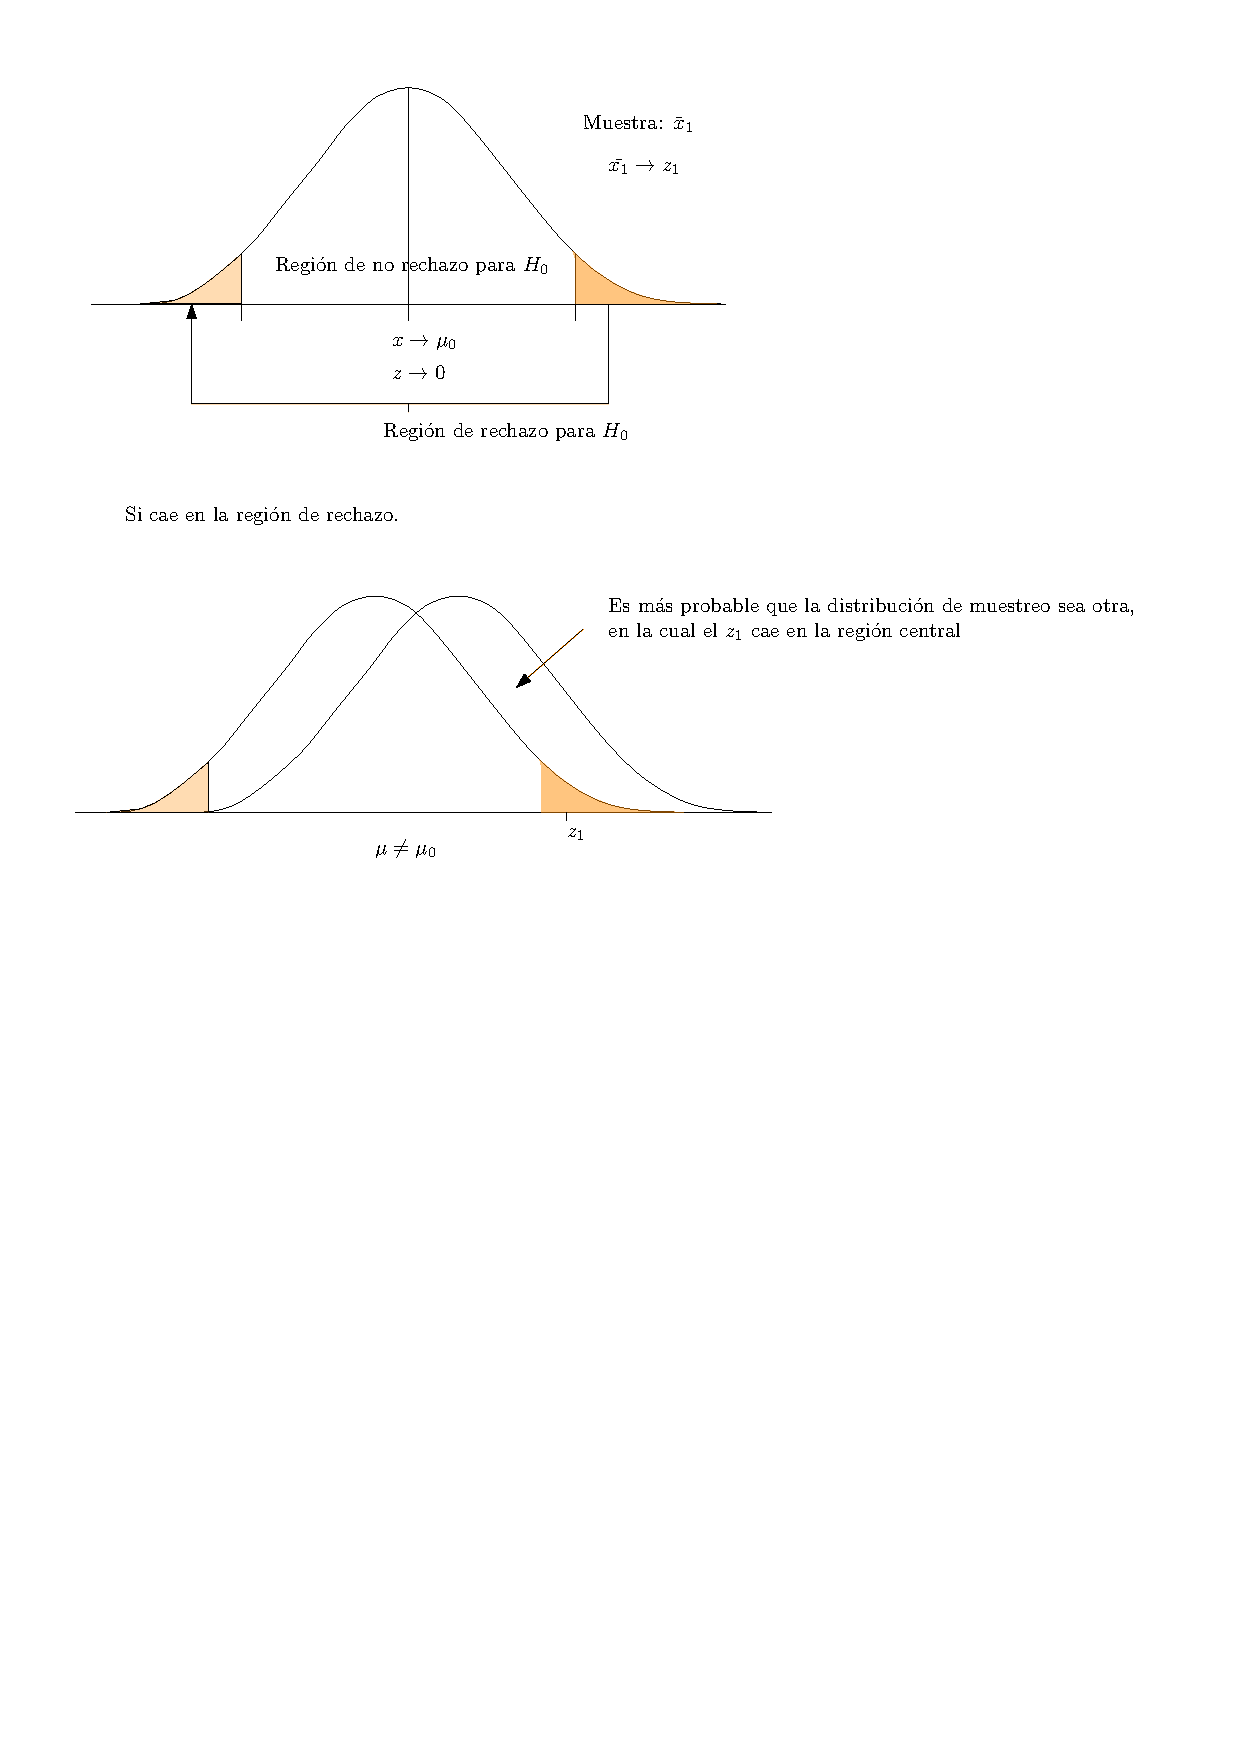
\includegraphics[width=14cm]{\figs/dist_29} 
        \end{figure}
    
    \item ¿Cuál es la probabilidad de error? $\alpha$ (significa la prueba) 
        \begin{itemize}
            \item $\alpha$: error tipo 1: rechazar $H_0$, cuando este era verdadero.
        \end{itemize}
    
    \item Si cae en la región de no rechazo: 
        \begin{figure}[H]
            \centering
            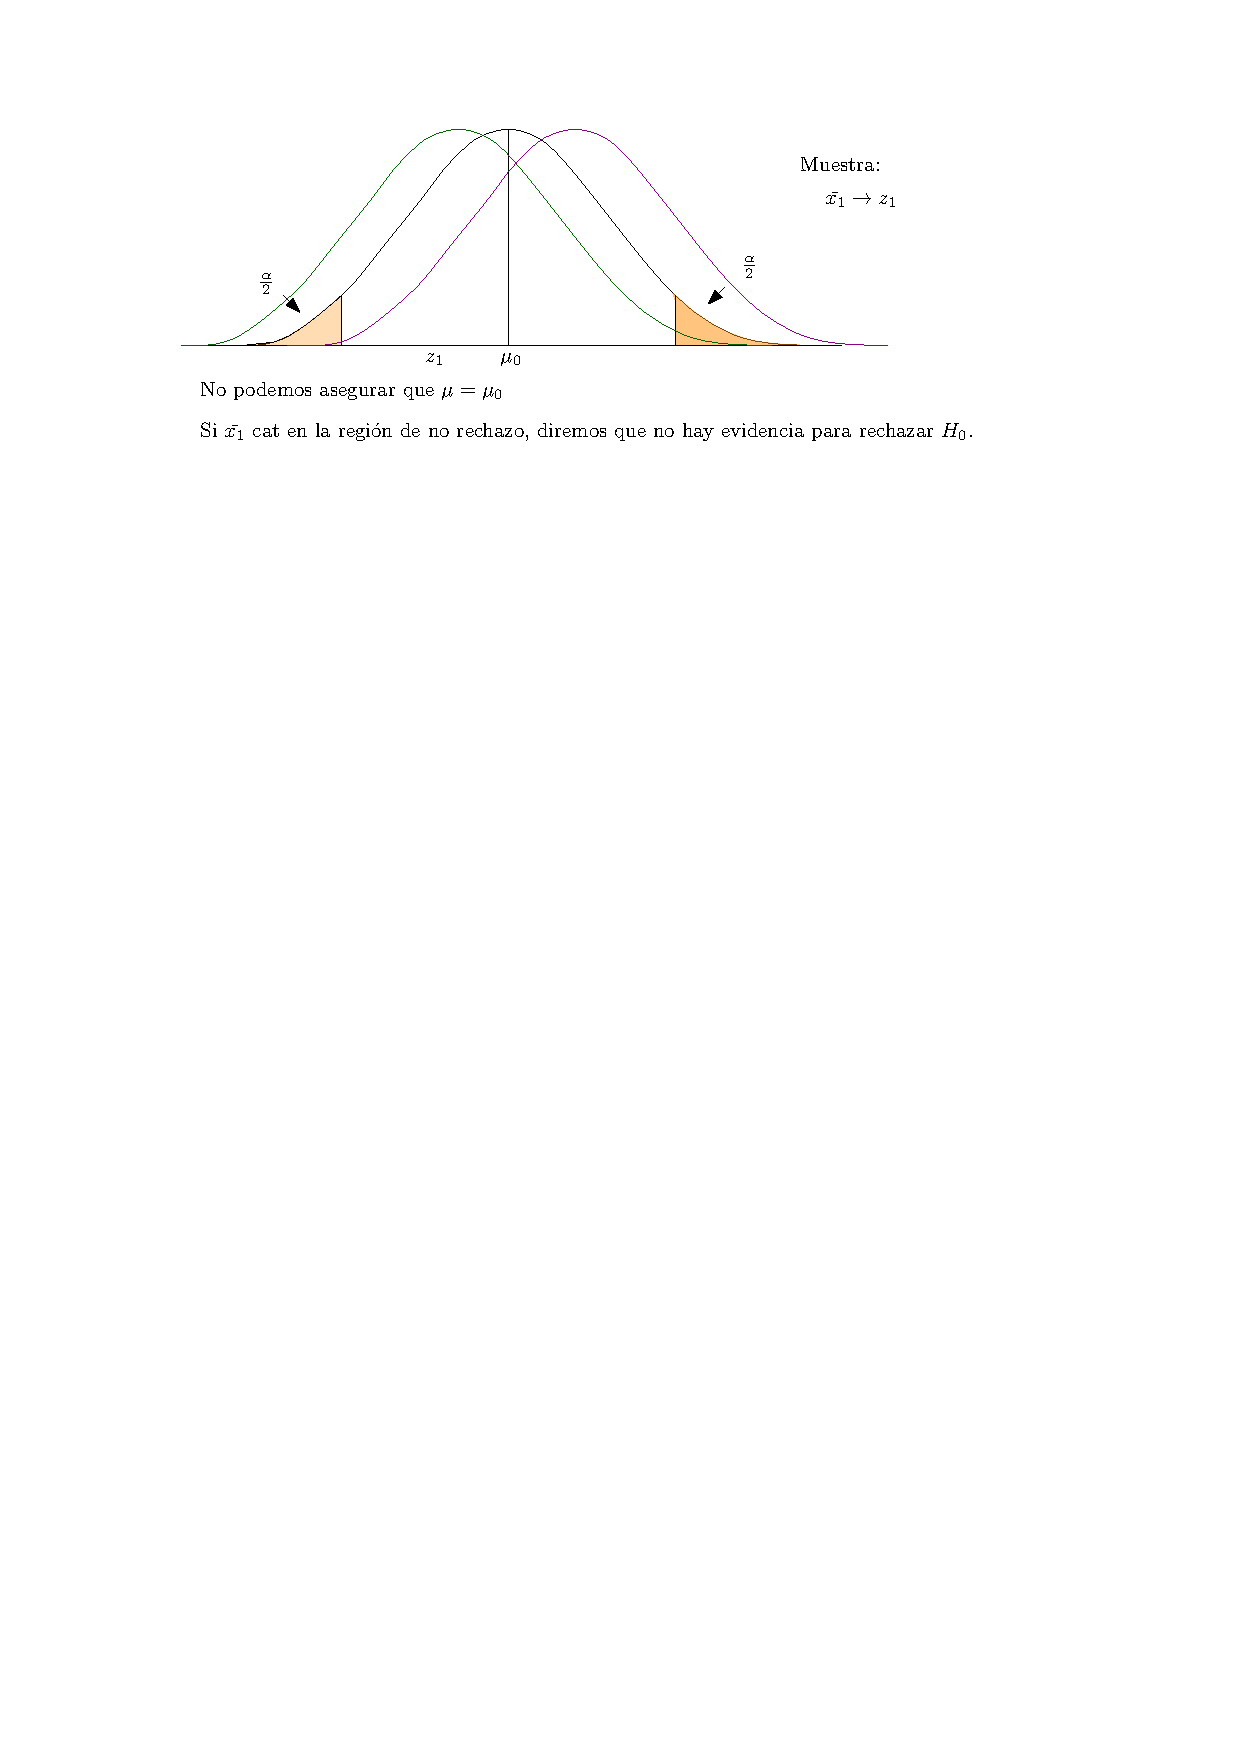
\includegraphics[width=14cm]{\figs/noevidence} 
        \end{figure}
    
    \item Dado a que estamos en un estado en el que no hay evidencia, a esto se le llama una conclusión débil.
        \begin{center}
           \begin{align*}
                \text{ La conclusión débil: } \qq & \text{ no rechazar $\mu_0$ } \\ 
                & \text{ Tipo de error: $\beta$  } \\ 
                & \text{ Error tipo 2: aceptar $H_0$  cuando este es falso.} \\  
                \\ 
                \text{ Conslusión fuerte: } \qq & \text{ Rechazar $H_0$  } \\ 
                & \text{ Tipo de error: $\alpha$ (controlado) } \\ 
                & \text{ Error tipo 1: Rechazar $H_0$ cuando este es verdadero.  } \\ 
           \end{align*}
        \end{center}
    
    \item Ya no hablemos del nivel de confianza si no de la significancia de la prueba, y eso es la probabilidad del error tipo uno y error controlado.
\end{itemize}

\section{Errores}
\begin{itemize}
    \item Ejemplo: usted es un juez y debe decidir si aplica la pena de muerte a un hombre acusado de violación. 
    \item Planteamos la hipótesis nula: 
        \begin{itemize}
            \item $H_0$: el acusado es culpable. 
            \item $H_a$: el acusado no es culpable. 
            \item El error tipo 1: (rechace la hipótesis nula, eso me lleva a aceptar la alternativa) Declaro al acusado inocente y lo dejo en libertad y si resulta que si era culpable. 
            \item El error tipo 2: lo declaro culpable y es inocente. 
        \end{itemize}
    
    \item Con el error tipo 2, si no llegue a rechazar la hipótesis nula lo que generalmente se hace es no tomar acción. 
    \item Planteemola al revés: 
        \begin{itemize}
            \item $H_0$: el acusado no es culpable.
            \item $H_a$: el acusado es culpable. 
            \item Error tipo 1: rechazar $H_0$ cuando esta era verdadera. Es decir, lo declaro culpable, cuando este era inocente. 
            \item Error tipo 2 ($\beta$): aceptar a $H_0$ cuando esta era falsa. Es decir, declararlo inocente siendo culpable. 
        \end{itemize}
\end{itemize}

\section{Ejercicios}
Plantear las hipótesis para los siguientes problemas.
\begin{enumerate}
    \item Acusan a nuestra empresa de estar robando, ya que aseguran que no damos las 100 lb que dice nuestro empaque. 
        \begin{itemize}
            \item Del lado del acusador: si nos enfocamos en la cantidad promedio. 
                \begin{itemize}
                    \item $H_0$: $\mu\geq 100$ 
                    \item $H_a$: $\mu < 100$ 
                \end{itemize}
        \end{itemize}
        \begin{figure}[H]
            \centering
            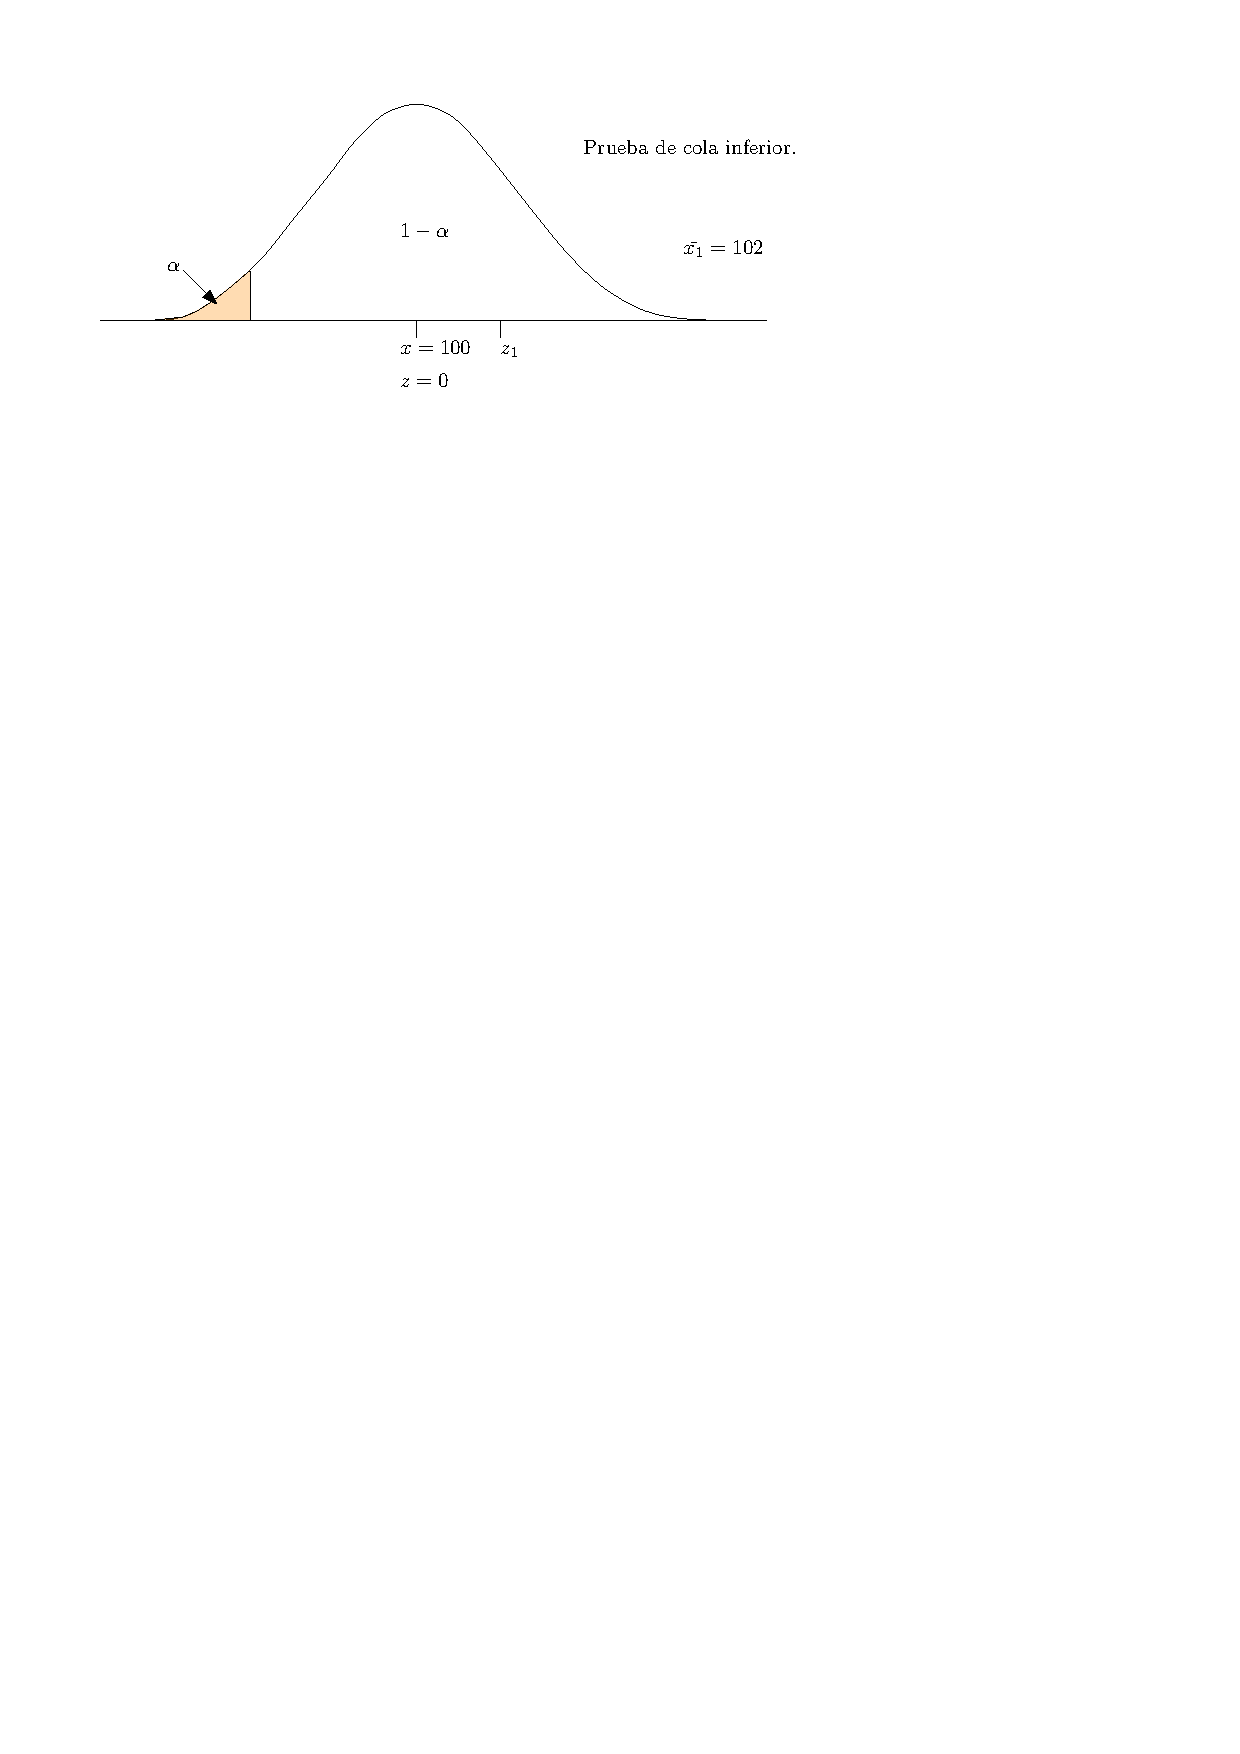
\includegraphics[width=14cm]{\figs/acusador} 
        \end{figure}
    
    \item Un planteamiento alterno podría ser el siguiente:
        \begin{itemize}
            \item $H_0$: $\mu\leq 100$ 
            \item $H_a$: $\mu> 100$ 
        \end{itemize}
        \begin{figure}[H]
            \centering
            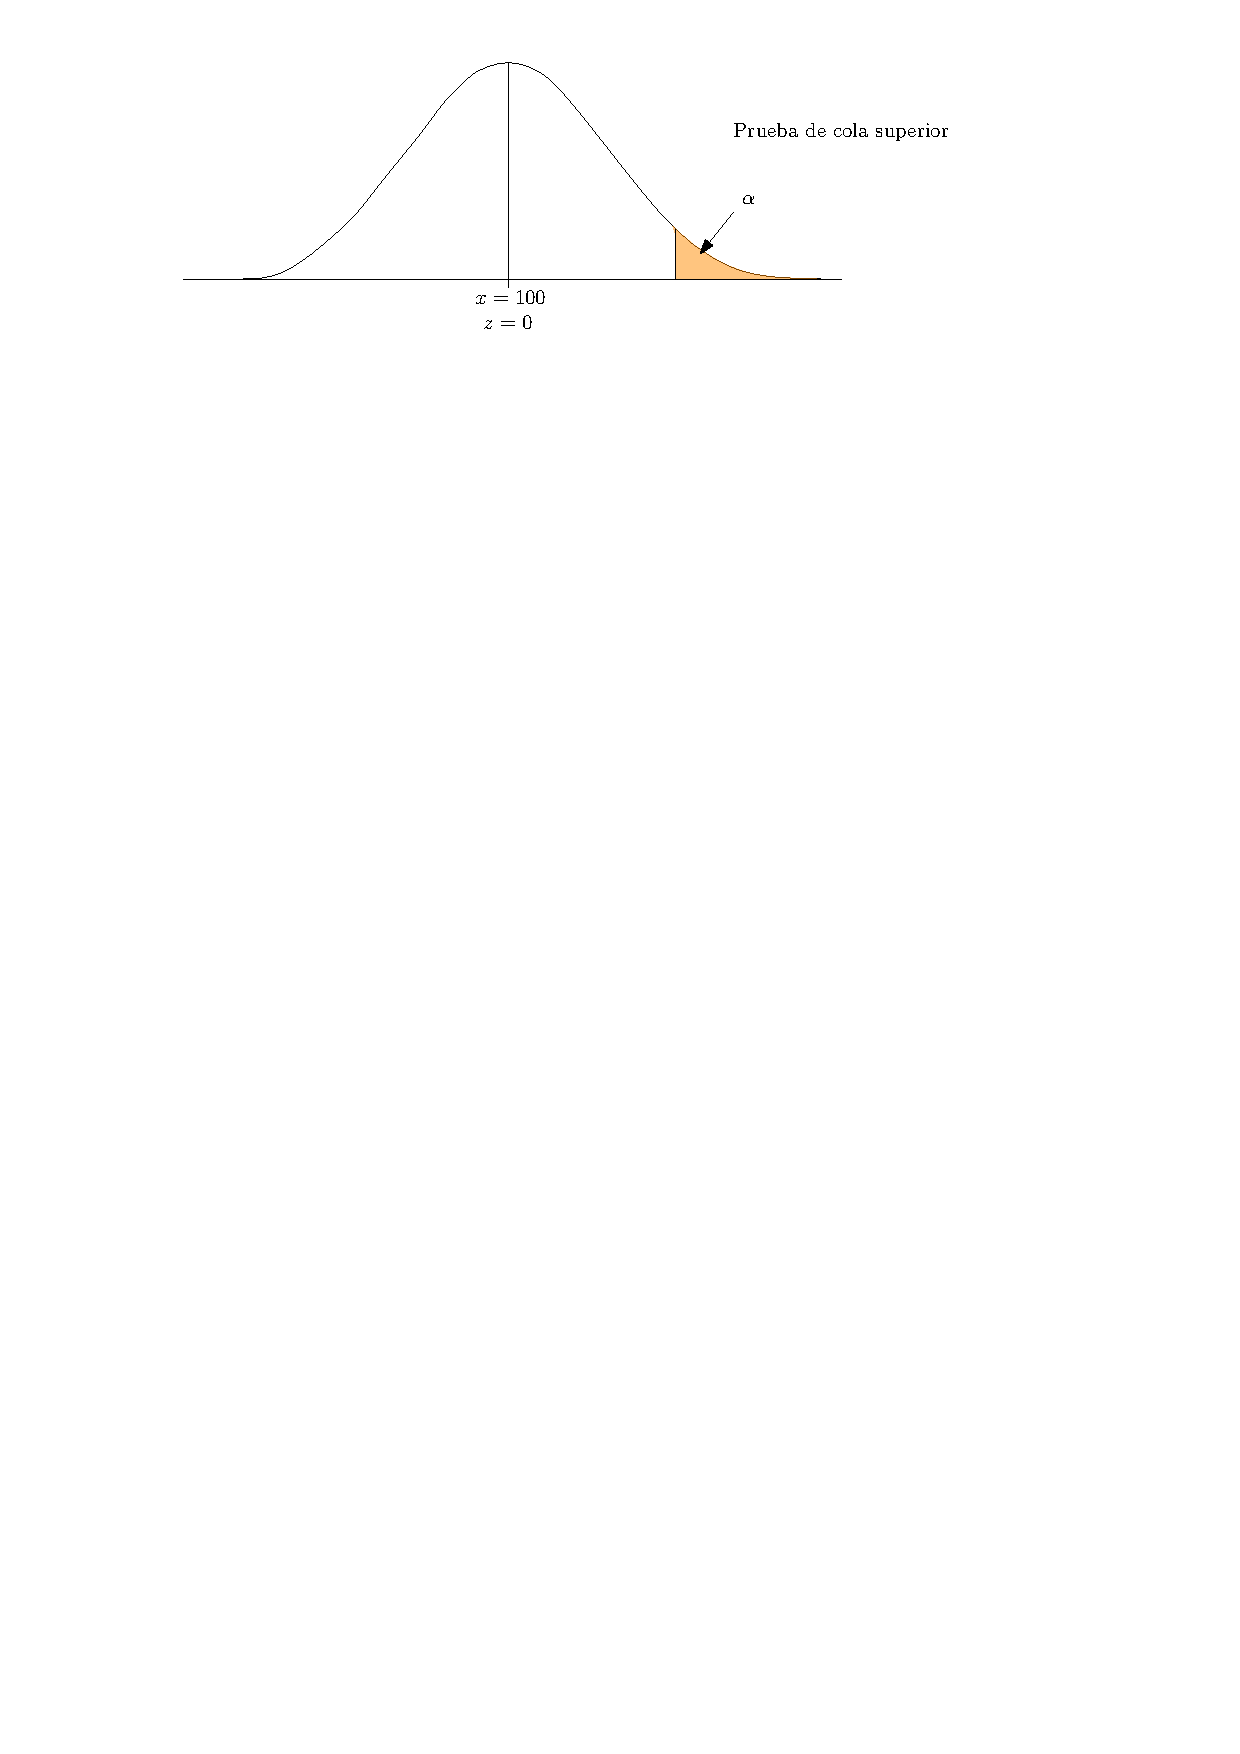
\includegraphics[width=14cm]{\figs/empresa} 
        \end{figure}
\end{enumerate}



\chapter{Bibliografía}
\begin{enumerate}
    \item Stephem Hawking: And God created the integers. 
    \item Carlos Castañeda: Las enseñanzas de don Juan.
    \item Leibniz: Dissertation on Combinatorial Art
    \item Leibniz: Monadología
    \item Terry Pinker: Hegel biography
    \item Cartas de la paz perpetua
\end{enumerate}

\chapter{Temas de interés}
\begin{itemize}
    \item Object-oriented ontology
    \item Tolstoy
\end{itemize}

%%%%%%%%%%%%%%%%%%%%%%%%%%%%%%%%%%%%%%%%%%%%%%%%%%%%%%%%%%%%%%%%%%%%%%%%%%%%%%%%%%%%%%%%%%%%%%%%%%%%%%%%%%%%%%%%%%%%%%%%%%%%%%%%%%%%%%%%%%%%%%
\end{document}

